\documentclass{beamer}

\usepackage{graphicx}
\usepackage[binary-units=true]{siunitx}

\title{Hardware Acceleration of Key-Value Stores}
\author{Sagar Karandikar, Howard Mao, Albert Ou, Soumya Basu}
\institute[UC Berkeley]{\textsc{University of California, Berkeley}}

\begin{document}
\frame{\titlepage}

\begin{frame}
    \frametitle{Introduction}

\begin{itemize}
    \item In datacenter applications, path through CPU / kernel / application
        accounts for 86\% of total request latency
    \item \textbf{Goal}: Serve popular requests without CPU interruption
    \item \textbf{Solution}: Hardware key-value store attached to the network
        interface controller
    \item Many workloads have an access pattern suitable for a small dedicated cache
        \begin{itemize}
            \item Per a Facebook study, 10\% of keys represent 90\% of requests
            \item Most values are relatively small in size (\SI{1}{\kilo\byte})
        \end{itemize}
\end{itemize}

\end{frame}

\begin{frame}{System Architecture}
    \includegraphics[width=\linewidth]{../img/system-kvstore.pdf}
\end{frame}

\begin{frame}{Accelerator}
    \includegraphics[width=\linewidth]{../img/kvstore.pdf}
\end{frame}

\begin{frame}{Traffic Manager}
    \includegraphics[width=\linewidth]{../img/frontend.pdf}
\end{frame}

\begin{frame}{DMA}
    \includegraphics[width=0.5\linewidth]{../img/dma-tx.pdf}
    \includegraphics[width=0.5\linewidth]{../img/dma-rx.pdf}
\end{frame}

\begin{frame}
    \frametitle{Design Space Exploration Parameters}

\begin{itemize}
    \item \texttt{wordsize} - The word size of the key memory. Affects the speed
        (cycle count) of key comparison.
        \begin{itemize}
            \item 8, 16, 32 (in Bytes)
        \end{itemize}
    \item \texttt{banksize} - The size of a single memory bank in the value memory.
        \begin{itemize}
            \item 128, 256 (in Bytes)
        \end{itemize}
    \item \texttt{maxfanin} - The number of bank values decoded in a single cycle in
        the key and value memory. Affects the depth of the memory pipeline.
        \begin{itemize}
            \item 8, 16
        \end{itemize}
    \item Clock Period:
        \begin{itemize}
            \item Minimum Clock Period - 0.75 ns (also roughly 10Gb Ethernet)
            \item 1Gb NIC Clock Period - 8 ns
%            \item 100Mb NIC Clock Period - 80 ns
        \end{itemize}
\end{itemize}

\end{frame}

\begin{frame}{Fixed Parameters}
    \begin{itemize}
        \item Many of these can be explored on FPGA - want to run with real traces
        \item \texttt{keysize}: 256B - Maximum allowed by memcached is 255
        \item \texttt{numkeys}: 64 - Number of lookup-slots for key-value pairs
        \item \texttt{valcachesize}: 32KiB - Size of space for values
        \item \texttt{countsize}: 4 - Width of hit-counters
    \end{itemize}
\end{frame}

\begin{frame}{Overview of DSE Results}
    \begin{itemize}
        \item Most parameters didn't have a significant effect
        \item Why?
    \end{itemize}
\end{frame}


\begin{frame}{Fixed ``Slow'' Clock (125 MHz)}

\noindent
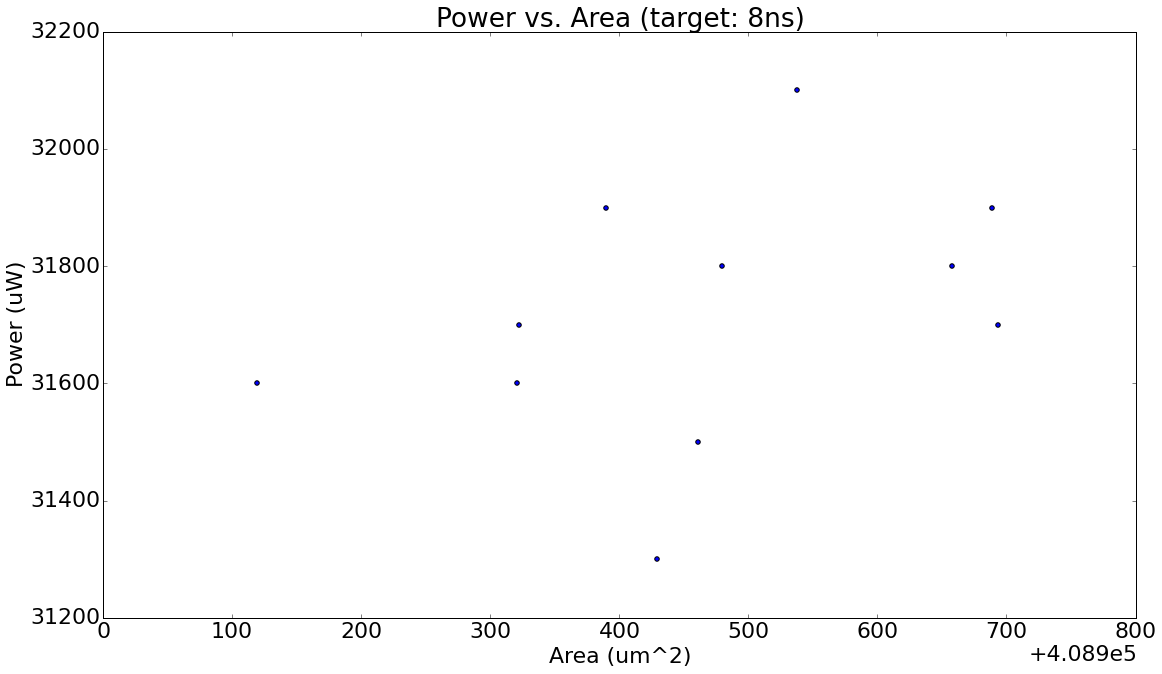
\includegraphics[width=0.4\textwidth]{../img/dse_slow/powerVSarea.png}\hspace{0.2\textwidth}%
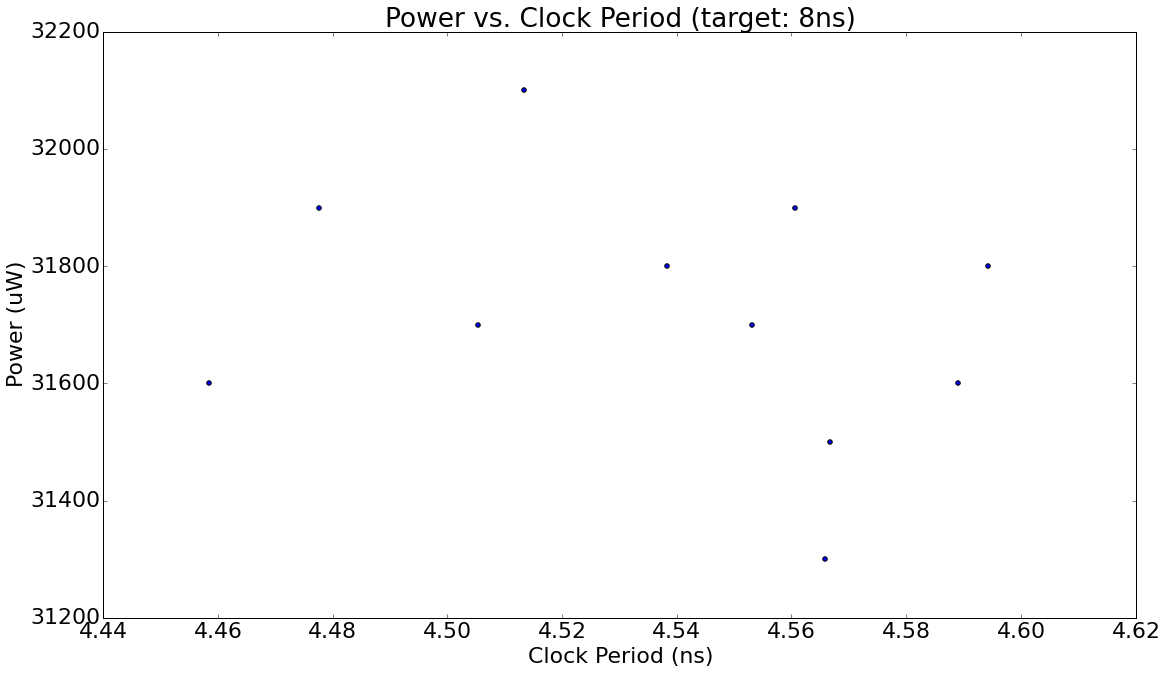
\includegraphics[width=0.4\textwidth]{../img/dse_slow/powerVSclock.png}\\[2em]
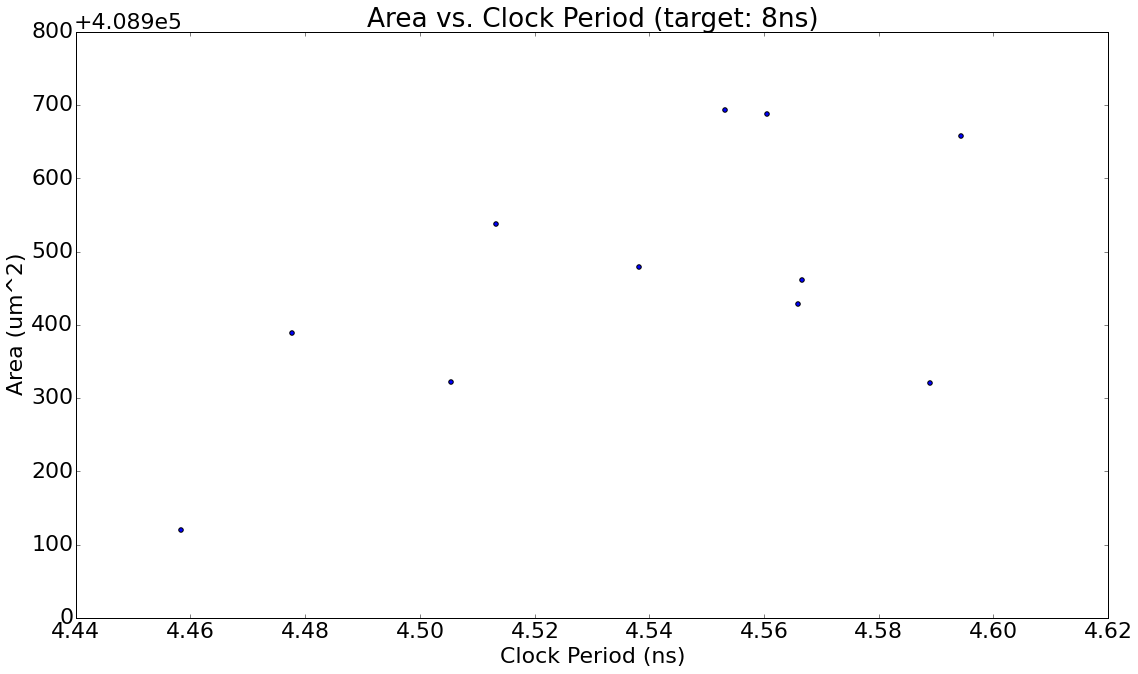
\includegraphics[width=0.4\textwidth]{../img/dse_slow/areaVSclock.png}\hspace{0.2\textwidth}%
%\includegraphics[width=0.4\textwidth]{four}\par 
    \tiny
    \begin{tabular}{c | c | c }
%Property & Mean & Std. Dev. \\ \hline
%Clock ($ns$) & 4.53843636364 & 0.042381047924  \\
%Power ($uW$) & 31718.1818182 & 208.100420768 \\
%Area ($um^{2}$) & 409363.605516 & 168.528457411 \\
Property & Mean & Std. Dev.  \\ \hline
Clock ($ns$) & 4.54 & 0.04 \\
Power ($uW$) & 31718.18 & 208.1 \\
Area ($um^2$) & 409364.0 & 169.0 \\
\end{tabular} \par
\end{frame}


\begin{frame}{Fixed ``Fast'' Clock (1.333 GHz)}
    \begin{itemize}
        \item show the cluster of points
    \end{itemize}
\end{frame}





\begin{frame}

    \frametitle{Full-System Evaluation}

\begin{itemize}
    \item 
    \item 
    \item 
\end{itemize}

\end{frame}



\begin{frame}
    \frametitle{Existing Infrastructure}

\begin{minipage}{0.4\linewidth}
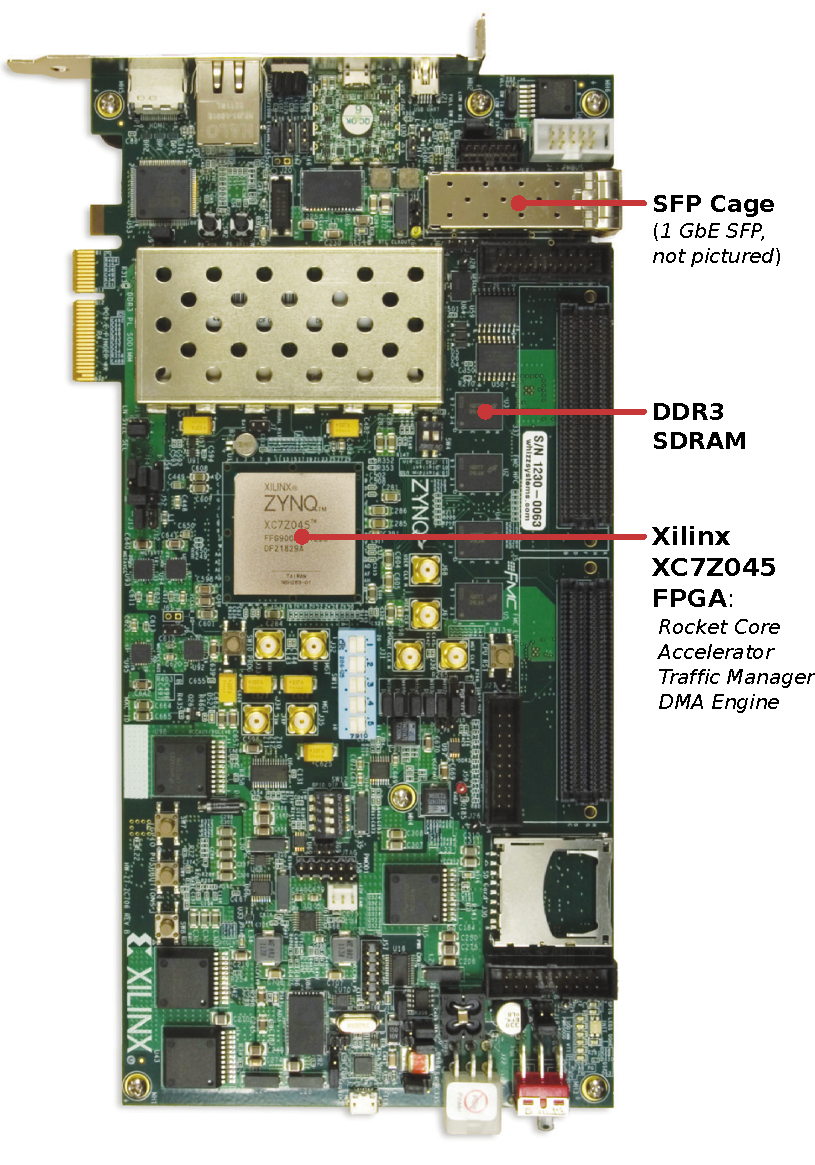
\includegraphics[width=\linewidth]{../img/zc706.pdf}
\end{minipage}
\hfill
\begin{minipage}{0.55\linewidth}
\alert{Xilinx ZC706 Evaluation Platform}
\begin{itemize}
\item ZYNQ-7000 SoC
\item Brocade 1GbE Copper SFP Transceiver
	\begin{itemize}
	\footnotesize
        \item Xilinx Tri-Mode Ethernet MAC
        \item Xilinx 1000Base-X PCS/PMA
	\end{itemize}
\item 64-bit RISC-V Rocket Core (\SI{50}{\mega\hertz})
	\begin{itemize}
	\footnotesize
	\item Single-issue, in-order, 6-stage pipeline
	\item ASIC version most nearly comparable with ARM Cortex-A5
	\end{itemize}
\end{itemize}
%\vspace{\baselineskip}
%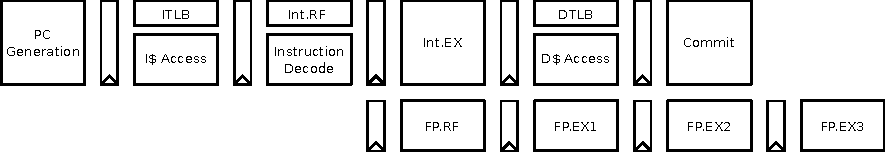
\includegraphics[width=\linewidth]{../img/rocket-pipeline.pdf}
\end{minipage}

\hrule
\vspace{0.5\baselineskip}
\begin{itemize}
\item No pre-existing I/O peripherals for the Rocket core
\end{itemize}
 




\end{frame}

\begin{frame}{Developing a NIC for RISC-V}
    \begin{itemize}
\item Built first RISC-V hardware device: register-mapped NIC
	\begin{itemize}
	\footnotesize
	\item Programmed I/O with custom Linux kernel driver
	\item First \texttt{telnet/ssh} session into a physical RISC-V machine
	\end{itemize}
\end{itemize}
\begin{center}
        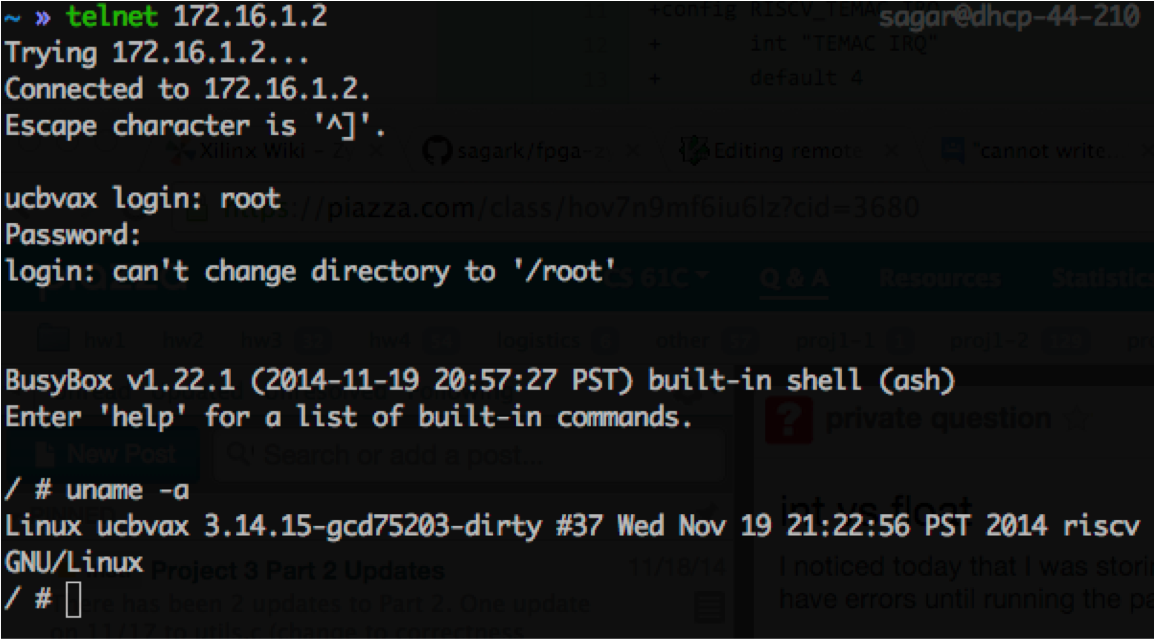
\includegraphics[scale=0.3]{../img/first_telnet.png}
    \end{center}

\begin{itemize}
\item Evolved to DMA-based NIC for performance
\end{itemize}
\end{frame}



\begin{frame}{Latency Comparison}
    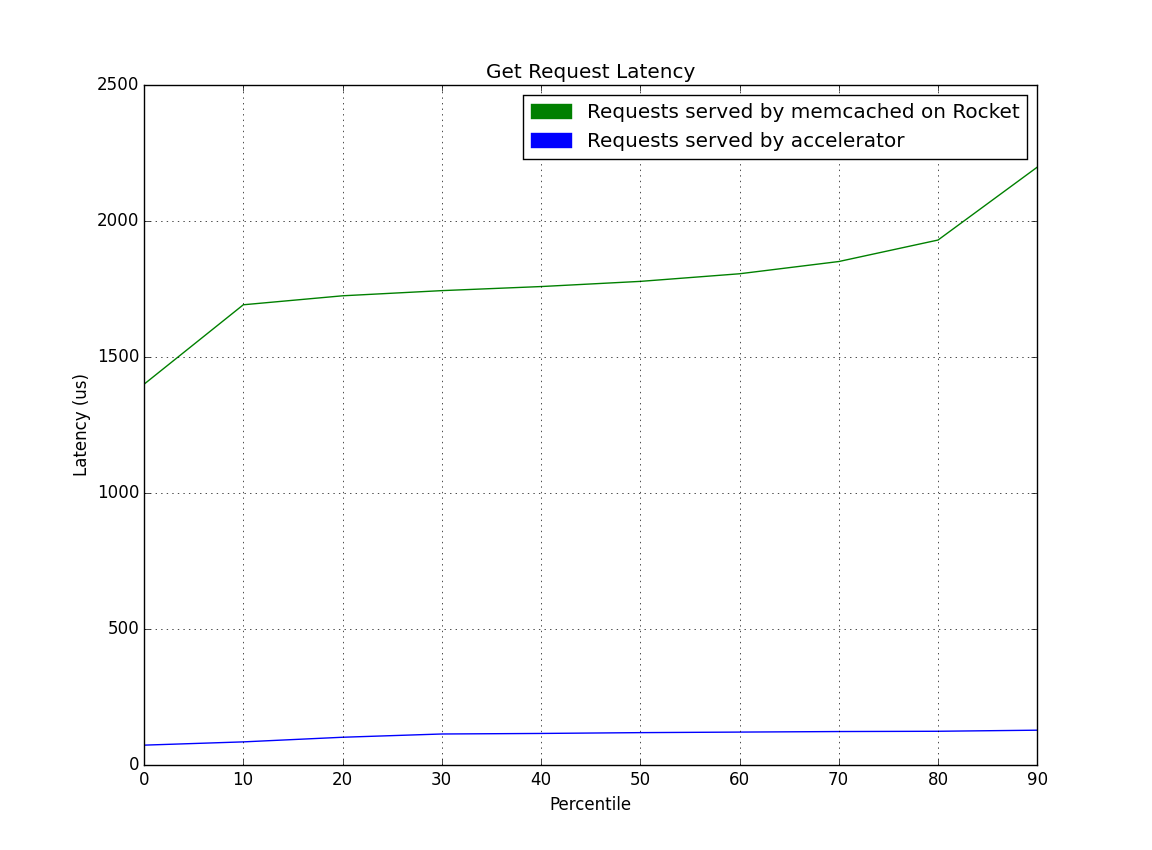
\includegraphics[width=\linewidth]{../img/graph.png}
\end{frame}

\begin{frame}
    Demo
\end{frame}

\end{document}
